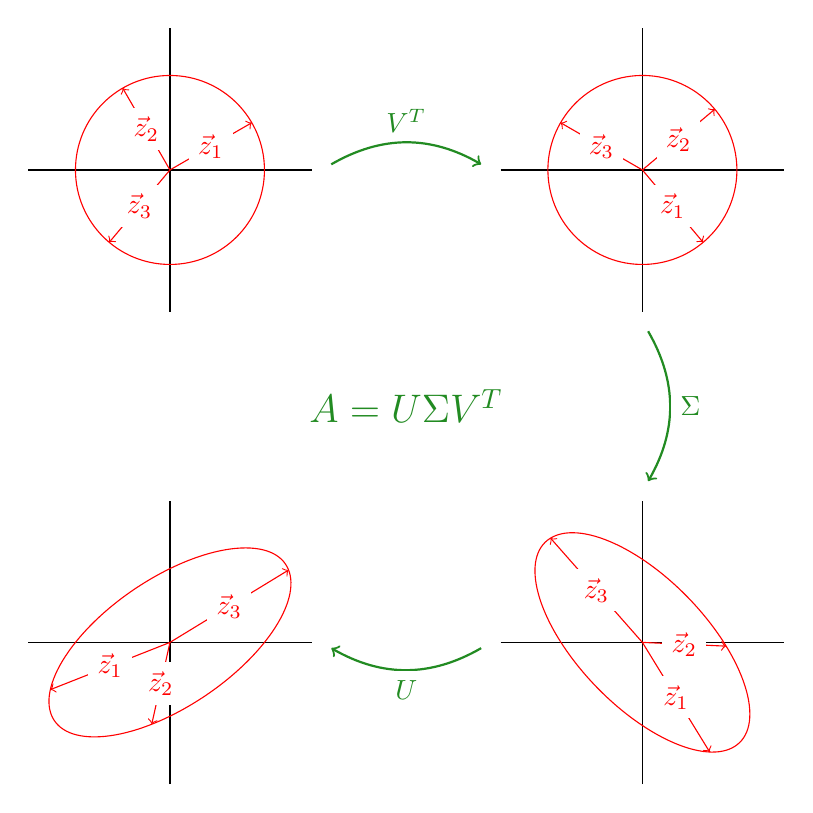
\begin{tikzpicture}[nodes={fill=white}, scale=1.2]
    \begin{scope}[xshift = 2.5cm, yshift=-2.5cm, ForestGreen, font=\Large]
        \node(){$A=U\Sigma V^T$};
    \end{scope}
    \begin{scope}
    \draw (-1.5, 0) -- (1.5, 0) node[right] (step1a){};
    \draw (0, -1.5) -- (0, 1.5);
    \begin{scope}[red]
    \draw (0, 0) circle (1);
    \draw[->] (0, 0) -- node[midway](){$\vec{z}_1$} (30:1);
    \draw[->] (0, 0) -- node[midway](){$\vec{z}_2$}(120:1);
    \draw[->] (0, 0) -- node[midway](){$\vec{z}_3$}(230:1);
    % \draw (0, 0) -- node[above](){$\vec{z}_1$} (30:1);
    % \draw (0, 0) -- node[left](){$\vec{z}_2$}(120:1);
    % \draw (0, 0) -- node[left](){$\vec{z}_3$}(230:1);
    \end{scope}
    \end{scope}
    \begin{scope}[xshift = 5cm]
        \draw (-1.5, 0) node[left](step1b){} -- (1.5, 0);
        \draw (0, -1.5) node[below](step2a){} -- (0, 1.5);
            \begin{scope}[rotate=-80, red]
                \draw (0, 0) circle (1);
    \draw[->] (0, 0) -- node[midway](){$\vec{z}_1$} (30:1);
    \draw[->] (0, 0) -- node[midway](){$\vec{z}_2$}(120:1);
    \draw[->] (0, 0) -- node[midway](){$\vec{z}_3$}(230:1);
            \end{scope}
    \end{scope}
    \begin{scope}[xshift = 5cm, yshift=-5cm]
        \draw (-1.5, 0) node[left](step3a){} -- (1.5, 0);
        \draw (0, -1.5) -- (0, 1.5) node[above](step2b){};
            \begin{scope}[red, rotate=-80, xslant=0.8]
                \draw (0, 0) circle (1);
    \draw[->] (0, 0) -- node[midway](){$\vec{z}_1$} (30:1);
    \draw[->] (0, 0) -- node[midway](){$\vec{z}_2$}(120:1);
    \draw[->] (0, 0) -- node[midway](){$\vec{z}_3$}(230:1);
            \end{scope}
    \end{scope}
    \begin{scope}[xshift = 0cm, yshift=-5cm]
        \draw (-1.5, 0) -- (1.5, 0) node[right](step3b){};
        \draw (0, -1.5) -- (0, 1.5);
            \begin{scope}[red, rotate=180, xslant=0.8]
                \draw (0, 0) circle (1);
    \draw[->] (0, 0) -- node[midway](){$\vec{z}_1$} (30:1);
    \draw[->] (0, 0) -- node[midway](){$\vec{z}_2$}(120:1);
    \draw[->] (0, 0) -- node[midway](){$\vec{z}_3$}(230:1);
            \end{scope}
    \end{scope}
    \draw[->,thick,  ForestGreen] (step1a) to[bend left] node[above](){$V^T$} (step1b);
    \draw[->, thick, ForestGreen] (step2a) to[bend left] node[right](){$\Sigma$} (step2b);
    \draw[->, thick, ForestGreen] (step3a) to[bend left] node[below](){$U$} (step3b);
\end{tikzpicture}
